\documentclass[aspectratio=169,usenames,dvipsnames]{beamer}
\usepackage{graphicx}
\usepackage{multimedia}
\usepackage{media9}
\usepackage{url}
\usepackage[algoruled,vlined,linesnumbered]{algorithm2e}
%\usepackage{amsmath}
%\usepackage{amssymb}
\usepackage{latexsym}
\usepackage{multirow}
\usepackage{comment}
\usepackage{wasysym}
\usepackage{units}
\usepackage{wrapfig}
\usepackage{extarrows}
\usepackage{diagbox}
\usepackage{qtree}
\usepackage{booktabs}

%%%%%%%%%%%% My packages %%%%%%%%%%%%%%%%%%%%%%%%%%%%
\usepackage[symbol]{footmisc}
\usepackage{booktabs}

%\usepackage{longtable}
%\usepackage{float}
%\usepackage{colortbl}
%\usepackage{threeparttable}
%\usepackage{tabu}

\usepackage{MnSymbol}

% bibliography
\usepackage[backend=bibtex,style=authoryear]{biblatex}
\addbibresource{bibliography0.bib}

% define slide theme
%\usetheme{Boadilla}
\usetheme{default}

% MATLAB colors: https://www.mathworks.com/help/matlab/ref/matlab.graphics.chart.primitive.histogram-properties.html
\definecolor{m1}{rgb}{0,0.4470,0.7410}
\definecolor{m2}{rgb}{0.8500,0.3250,0.0980}
\definecolor{m3}{rgb}{0.9290,0.6940,0.1250}
\definecolor{m4}{rgb}{0.4940,0.1840,0.5560}
\definecolor{m5}{rgb}{0.4660,0.6740,0.1880}
\definecolor{m6}{rgb}{0.3010,0.7450,0.9330}
\definecolor{m7}{rgb}{0.6350,0.0780,0.1840}

\newcommand{\tcb}[1]{\textcolor{m1}{#1}}
\newcommand{\tco}[1]{\textcolor{m2}{#1}}
\newcommand{\tcv}[1]{\textcolor{m4}{#1}}
\newcommand{\tcg}[1]{\textcolor{m5}{#1}}
\newcommand{\tcm}[1]{\textcolor{m7}{#1}}

% define the heading color
\definecolor{myorange}{rgb}{0.807,0.3137,0.047}
\makeatletter
\colorlet{beamer@blendedblue}{myorange}
\makeatother

\definecolor{gray75}{gray}{0.75}

% define the footer
\definecolor{gray50}{gray}{0.5}
\setbeamertemplate{footline}[text line]{%
\parbox{\linewidth}{\vspace*{-8pt}\textcolor{gray50}{\inserttitle\hfill\insertpagenumber}}}

% get rid of the navigations symbols at the bottom
\setbeamertemplate{navigation symbols}{}

% custom font
%\usepackage{heuristica}
%\usepackage[heuristica,vvarbb,bigdelims]{newtxmath}
%\usepackage[T1]{fontenc}
%\renewcommand*\oldstylenums[1]{\textosf{#1}}
% More fonts here: http://www.tug.dk/FontCatalogue/mathfonts.html

%\usepackage[default]{comfortaa}
%\usepackage[T1]{fontenc}

\usepackage[sfdefault,light]{roboto}  
\usepackage[T1]{fontenc}


%%%%%%%%%%%%% Vadim's macro definitions %%%%%%%%%%%%%%%%%%

\newtheorem{df}{Definition}
\newtheorem{notation}{Notation}
\newtheorem{col}{Corollary}
\newtheorem{lem}{Lemma}

\newcommand{\td}{\,\nicefrac{\times}{\div}\,}

\newcommand{\bt}{\begin{theorem}\em}
\newcommand{\et}{\end{theorem}}
\newcommand{\Qed}{$\blacksquare$}
\renewcommand{\nin}{\noindent}
\newcommand{\bea}{\begin{eqnarray}}
\newcommand{\eea}{\end{eqnarray}}
\newcommand{\bdf}{\begin{df}\em}
\newcommand{\edf}{\end{df}}

\newcommand{\ben}{\begin{enumerate}}
\newcommand{\een}{\end{enumerate}}
\newcommand{\bei}{\begin{itemize}}
\newcommand{\eei}{\end{itemize}}
\newcommand{\ie}{\item}

\newcommand{\midb}{\pmb{\mid}}

\newcommand{\dist}{\operatorname{dist}}
\newcommand{\avg}{\operatornamewithlimits{avg}\limits}
\renewcommand{\arg}{\operatornamewithlimits{arg}\limits}
\newcommand{\round}{\operatorname{round}}
\newcommand{\lop}{\operatorname{lop}}
%\renewcommand{\min}{\operatornamewithlimits{argmin}\limits}
\renewcommand{\max}{\operatornamewithlimits{max}\limits}
\newcommand{\median}{\operatornamewithlimits{median}\limits}
\newcommand{\mean}{\operatornamewithlimits{mean}\limits}
\newcommand{\argmax}{\operatornamewithlimits{argmax}\limits}
\newcommand{\argmin}{\operatornamewithlimits{argmin}\limits}

\numberwithin{equation}{section}
\numberwithin{theorem}{section}
\numberwithin{lem}{section}
\numberwithin{df}{section}

\newcommand{\citea}[1]
{\citeauthor{#1} (\citeyear{#1})}

\setbeamerfont{caption}{series=\normalfont,size=\fontsize{6}{6}}
\definecolor{gray75}{gray}{0.75}
\setbeamertemplate{caption}{\raggedright\textcolor{myorange}{\insertcaption}\par}

\begin{document}

\title{Core Expansion in Optimization Crosswords}
\author{Adi Botea and Vadim Bulitko}
\institute{Eaton \& University of Alberta} 
%\institute{
\includegraphics[width=0.2\textwidth]{_template/uofa.pdf}} 

\date{July 14, 2023}

\frame{\titlepage} 

%%%%%%%%%%%%%%%%%%%%%%%%%%%%%%%%%%%%%%%%%%%%%%%%%%%%%%%%%%%%%%%%%%%%%%%%%%%%%%%%

\begin{frame}{Outline}

\bei

\ie Heuristic Search

\bigskip

\ie Synthesis of Heuristic Functions

\bigskip

\ie Results

\bigskip

\ie Current Shortcomings \& Future Work

\bigskip

\ie Conclusions

\eei

\end{frame}

%%%%%%%%%%%%%%%%%%%%%%%%%%%%%%%%%%%%%%%%%%%%%%%%%%%%%%%%%%%%%%%%%%%%%%%%%%%%%%%%

\begin{frame}{Heuristic Search}

\begin{columns}
\column{0.6\linewidth}


\bei

\ie For pathfinding%~[\cite{sturtevant2019pathfinding}]

\bei

\ie guided by heuristic

\eei

\medskip

\ie Common heuristics 

\bei

\ie human-designed (e.g., $\Delta x + \Delta y$)

\bei

\ie \tcg{little memory}

\ie \tcg{portable}

\ie \tcg{easy to communicate to humans}

\ie \tcm{low performance}

\eei

\ie pre-computed~[\cite{conf/ijcai/SturtevantFBSB09}]

\bei

\ie \tcm{substantial memory}

\ie \tcm{map-specific}

\ie \tcm{difficult to communicate to humans}

\ie \tcg{high performance}

\eei

\eei 

\medskip

\ie Combine the \tcg{best} of both?

\eei

\column{0.4\linewidth}
\begin{figure}[tbp]
\centering

\includegraphics[height=5cm]{figs/mce.png}
\end{figure}
\end{columns} 



\end{frame}


%%%%%%%%%%%%%%%%%%%%%%%%%%%%%%%%%%%%%%%%%%%%%%%%%%%%%%%%%%%%%%%%%%%%%%%%%%%%%%%%

\begin{frame}{Problem Formulation: Synthesis of Heuristic Functions}

\bei

\ie Find $h^{\min}$ that minimizes the {\em loss} $\ell$ of the search algorithm $a$ guided by the heuristic $h$ over search problems $P$:
\bea 
h^{\min} = \argmin\limits_{h \in \mathcal{H}}  \ell(a,h,P) \nonumber 
\eea
where:
\bei

\ie $\mathcal{H}$ is a space of heuristics

\ie loss $\ell$ is the ratio of the number of states expanded by $a$ and $h$ to that of the baseline for the same solution quality
\bei
\ie $\ell = \nicefrac{1}{2}$ means that $(a,h)$ matched the solution quality of the baseline yet expanded half the number of states
\eei

\eei

\eei 

\end{frame}

%%%%%%%%%%%%%%%%%%%%%%%%%%%%%%%%%%%%%%%%%%%%%%%%%%%%%%%%%%%%%%%%%%%%%%%%%%%%%%%%

\begin{frame}{Problem Formulation: Portability}

\bei

\ie {\em Degradation} of heuristic $h$ performance:
\bea  
\mathcal{D}(a,P,h_P,P',h_{P'}) = \ell(h_P,a,P') - \ell(h_{P'},a,P') \nonumber
\eea
where:
\bei
\ie heuristic $h_P$ synthesized $P$
\ie heuristic $h_{P'}$ synthesized $P'$
\ie $\ell(h_P,a,P')$ computed on $P'$ and compared to $\ell(h_{P'},a,P')$ 
\eei 

\bigskip

\ie Low degradation means high {\em portability} of the heuristic

\eei 

\end{frame}


%%%%%%%%%%%%%%%%%%%%%%%%%%%%%%%%%%%%%%%%%%%%%%%%%%%%%%%%%%%%%%%%%%%%%%%%%%%%%%%%

\begin{frame}{Desired Solution Properties}

\bei

\ie Automated synthesis
\bei
\ie from a single commodity computer to a cluster
\eei

\medskip

\ie Low loss
\bei
\ie high portability across video-game maps
\ie low memory cost
\eei

\medskip

\ie Human readability
\bei
\ie how/why synthesized heuristics work
\ie theoretical bounds
\eei


\eei 

\end{frame}


%%%%%%%%%%%%%%%%%%%%%%%%%%%%%%%%%%%%%%%%%%%%%%%%%%%%%%%%%%%%%%%%%%%%%%%%%%%%%%%%

\begin{frame}{Related Work I}

\bei

\ie Memory-based heuristics~[\cite{PDB,felner2007compressed,conf/aiide/BjornssonH06,conf/ijcai/SturtevantFBSB09}]
\bei
\ie \tcm{high memory cost, no human readability, no portability}
\eei

\medskip

\ie Compressed solutions~[\cite{botea2011ultra,botea2013path}]
\bei
\ie \tcm{high memory cost, no human readability, no portability}
\eei

\medskip

\ie Embedding into a Euclidean space so that Euclidean distance can be used as the heuristic~[\cite{rayner2011euclidean,cohenfastmap}]
\bei
\ie \tcm{no human readability, no portability}
\eei

\eei

\end{frame}

%%%%%%%%%%%%%%%%%%%%%%%%%%%%%%%%%%%%%%%%%%%%%%%%%%%%%%%%%%%%%%%%%%%%%%%%%%%%%%%%

\begin{frame}{Related Work II}

\bei



\ie Learning heuristic functions~[\cite{samadi2008learningFrom,biss_aij,agostinelli2019rubik,orseauL21}]
\bei
\ie \tcm{no human readability}
\eei

\bigskip

\ie Program synthesis for heuristic search {\em algorithms}~[\cite{bulitkoAlife2016,bulitkoSoCSalife2016}]
\bei
\ie \tcb{complimentary to our approach}
\eei

\eei

\end{frame}

%%%%%%%%%%%%%%%%%%%%%%%%%%%%%%%%%%%%%%%%%%%%%%%%%%%%%%%%%%%%%%%%%%%%%%%%%%%%%%%%

\begin{frame}{Building On Our Previous Work}

\bei

\ie Our previous work~[\cite{cog2021short}]

\bigskip
\bigskip

\ie \tcg{Advances/contributions of this paper}
\bei

\medskip

\ie {\bf new algorithm} unifies and generalizes the stochastic sampling, simulated annealing and a genetic algorithm
\bei
\ie the last two can {\em accumulate} modifications over time $\to$ more complex heuristic formula $\to$ possibly capture more specifics of a search graph
\eei

\medskip

\ie {\bf analysis:} a commonly synthesized heuristic; bounds

\medskip


\ie {\bf portability}: synthesized heuristics across different search graphs
\bei
\ie heuristics synthesized for one game outperform the baseline on a different game
\eei 

\eei

\eei

\end{frame}


%%%%%%%%%%%%%%%%%%%%%%%%%%%%%%%%%%%%%%%%%%%%%%%%%%%%%%%%%%%%%%%%%%%%%%%%%%%%%%%%

\begin{frame}{Our Approach: Intuition}

\bei

\ie To help with low memory cost, human readability and portability
\bei
\ie \tcv{a space of algebraic formulae defined by a context-free grammar}
\eei

\bigskip

\ie Synthesis via stochastic search through the space of such formulae
\bei
\ie \tcv{stochastic sampling}
\ie \tcv{accumulating mutations}
\ie \tcv{probabilistic acceptance}
\ie \tcv{population of promising formulae}
\ie \tcv{progressive evaluation}
\ie \tcv{previously synthesized formulae as building blocks}
\eei

\eei

\end{frame}

%%%%%%%%%%%%%%%%%%%%%%%%%%%%%%%%%%%%%%%%%%%%%%%%%%%%%%%%%%%%%%%%%%%%%%%%%%%%%%%%

\begin{frame}{Our Approach: Space of Initial Heuristics $\mathcal{H}$}

\begin{columns}
\column{0.6\linewidth}

\bei

\ie A heuristic is a formula: $h(x,y,x_g,y_g) = F$ defined by this grammar:

{\small\bea
F &\to& T \midb U \midb B \nonumber \\
T &\to& x \midb x_g \midb y \midb y_g \midb \Delta x \midb \Delta y \midb C \nonumber  \\
U &\to& \sqrt{F} \midb |F| \midb -F \midb F^2 \nonumber \\
B &\to& F+F \midb F-F \midb F \times F \midb \frac{F}{F} \midb \max\{F,F\} \midb \min\{F,F\} \nonumber 
\eea}

\nin here $\Delta x = |x - x_g|$, $\Delta y = |y - y_g|$ and $C \in \{1.0, 1.1, 1.2, \dots, 10.0\}$

\eei

\column{0.4\linewidth}
\begin{figure}[htbp]
\vspace{-0.25cm}
\Tree [.$\times$ $5$ [.$+$ $\Delta x$ $\Delta y$ ] ]
\caption{Manhattan distance weighted by $5$}
\label{fig:weightedMD}
\end{figure}
\end{columns} 




\end{frame}


%%%%%%%%%%%%%%%%%%%%%%%%%%%%%%%%%%%%%%%%%%%%%%%%%%%%%%%%%%%%%%%%%%%%%%%%%%%%%%%%

\begin{frame}{Empirical Evaluation}

\bei

\ie 2D grid pathfinding~[\cite{sturtevant2012benchmarks}]

\bigskip

\ie $24$ maps from two games:
\bei
\ie {\em Dragon Age: Origins} ({\tt DAO})
\ie {\em StarCraft} ({\tt SC}) 
\eei

\bigskip

\ie To study portability: two sets of six maps each from each game
\bei
\ie {\tt DAO-A}
\ie {\tt DAO-B}
\ie {\tt SC-A}
\ie {\tt SC-B}
\eei

\eei


\end{frame}


%%%%%%%%%%%%%%%%%%%%%%%%%%%%%%%%%%%%%%%%%%%%%%%%%%%%%%%%%%%%%%%%%%%%%%%%%%%%%%%%

\begin{frame}{Loss}

\bei

\ie computed with respect to a baseline~[\cite{cog2021short}]
\bei
\ie weighted A* with Manhattan Distance
\ie interpolated, averaged
\eei

\bigskip

\ie regularized during synthesis:
\bea
\ell^\lambda(a,h,P) = \ell(a,h,P) + \lambda |h|\nonumber
\eea 
here $|h|$ is the number of vertices in the syntax tree representing the heuristic $h$; $\lambda$ is the regularizer constant

\eei


\end{frame}


%%%%%%%%%%%%%%%%%%%%%%%%%%%%%%%%%%%%%%%%%%%%%%%%%%%%%%%%%%%%%%%%%%%%%%%%%%%%%%%%

\begin{frame}{Synthesis: Base Grammar: {\tt DAO-A}}

\begin{table}[htbp]
 \setlength{\tabcolsep}{3pt}
	\centering
	{
		\begin{tabular}{c|l}
			\toprule
			{\bf Test loss} & {\bf Heuristic}\\
			\midrule
			$0.4007$ & 
			$\mathbf{f_{1}} = \max\left\{\Delta x \cdot \sqrt{\frac{y_g}{x}},\Delta y\right\}^4$\\
			$0.3627$ & 
			$\mathbf{f_{2}} = \Delta y + 44.9 \cdot \max\left\{\Delta x,\Delta y\right\}$\\
			$0.4494$ & 
			$\mathbf{f_{3}} = \max\left\{\frac{y_g}{\left(y - 8.3\right)} \cdot \Delta y,\Delta x\right\}^2$\\
			$0.4995$ & 
			$\mathbf{f_{4}} = \max\left\{100.0,\min\left\{y_g,\Delta y\right\} + y\right\}^2 \cdot \max\left\{\Delta x,\Delta y\right\}$\\
			$0.4894$ & 
			$\mathbf{f_{5}} = \max\left\{\sqrt{\left(y + \Delta y\right)^2 \cdot \Delta y} \cdot 11.5,\Delta x \cdot y_g\right\}$\\
			$0.4798$ & 
			$\mathbf{f_{6}} = \max\left\{\Delta y,\Delta x + \min\left\{\Delta x,x_g\right\}\right\}^2$\\
			\bottomrule
		\end{tabular}}
	\caption{Synthesized heuristics for maps {\tt brc202d}, {\tt den000d}, {\tt den501d}, {\tt lak505d}, {\tt orz103d}, {\tt ost000a} in {\tt DAO-A}, manually simplified for readability}
	\label{tab:building_blocks_from_DAO-A}
\end{table}


\end{frame}

%%%%%%%%%%%%%%%%%%%%%%%%%%%%%%%%%%%%%%%%%%%%%%%%%%%%%%%%%%%%%%%%%%%%%%%%%%%%%%%%

\begin{frame}{Synthesis: Base Grammar: {\tt SC-A}}

\begin{table}[htbp]
	\centering
	{
		\begin{tabular}{c|l}
			\toprule
			{\bf Test loss} & {\bf Heuristic}\\
			\midrule
			$0.2846$ & 
			$\mathbf{f_{7}} = \max\left\{\Delta y,\Delta x\right\} \cdot x_g + \Delta y$\\
			$0.3539$ & 
			$\mathbf{f_{8}} = \max\left\{\sqrt{y} + \Delta y,\Delta x\right\}^2 + \Delta y$\\
			$0.4711$ & 
			$\mathbf{f_{9}} = \Delta x + \max\left\{\Delta y \cdot 5.6,\Delta x\right\}$\\
			$0.3310$ & 
			$\mathbf{f_{10}} = \max\left\{\Delta y \cdot \sqrt{\sqrt{\sqrt{\Delta y}}},\Delta x\right\}^2 - \Delta y + \Delta x$\\
			$0.4931$ & 
			$\mathbf{f_{11}} = \Delta x + \max\left\{1.5 \cdot \Delta y,\Delta x\right\} \cdot 5.6$\\
			$0.2679$ & 
			$\mathbf{f_{12}} = \max\left\{\Delta y + \sqrt{y_g},\Delta x\right\}^2$\\
			\bottomrule
		\end{tabular}}
	\caption{Synthesized heuristics for maps {\tt Legacy}, {\tt Rosewood}, {\tt ShroudPlatform}, {\tt SpaceAtoll},  {\tt Triskelion}, {\tt WarpGates} in {\tt SC-A}, manually simplified for readability}
	\label{tab:building_blocks_from_SC-A}
\end{table}


\end{frame}

%%%%%%%%%%%%%%%%%%%%%%%%%%%%%%%%%%%%%%%%%%%%%%%%%%%%%%%%%%%%%%%%%%%%%%%%%%%%%%%%

\begin{frame}{Performance Gains}

\begin{figure}[htbp]
\centering
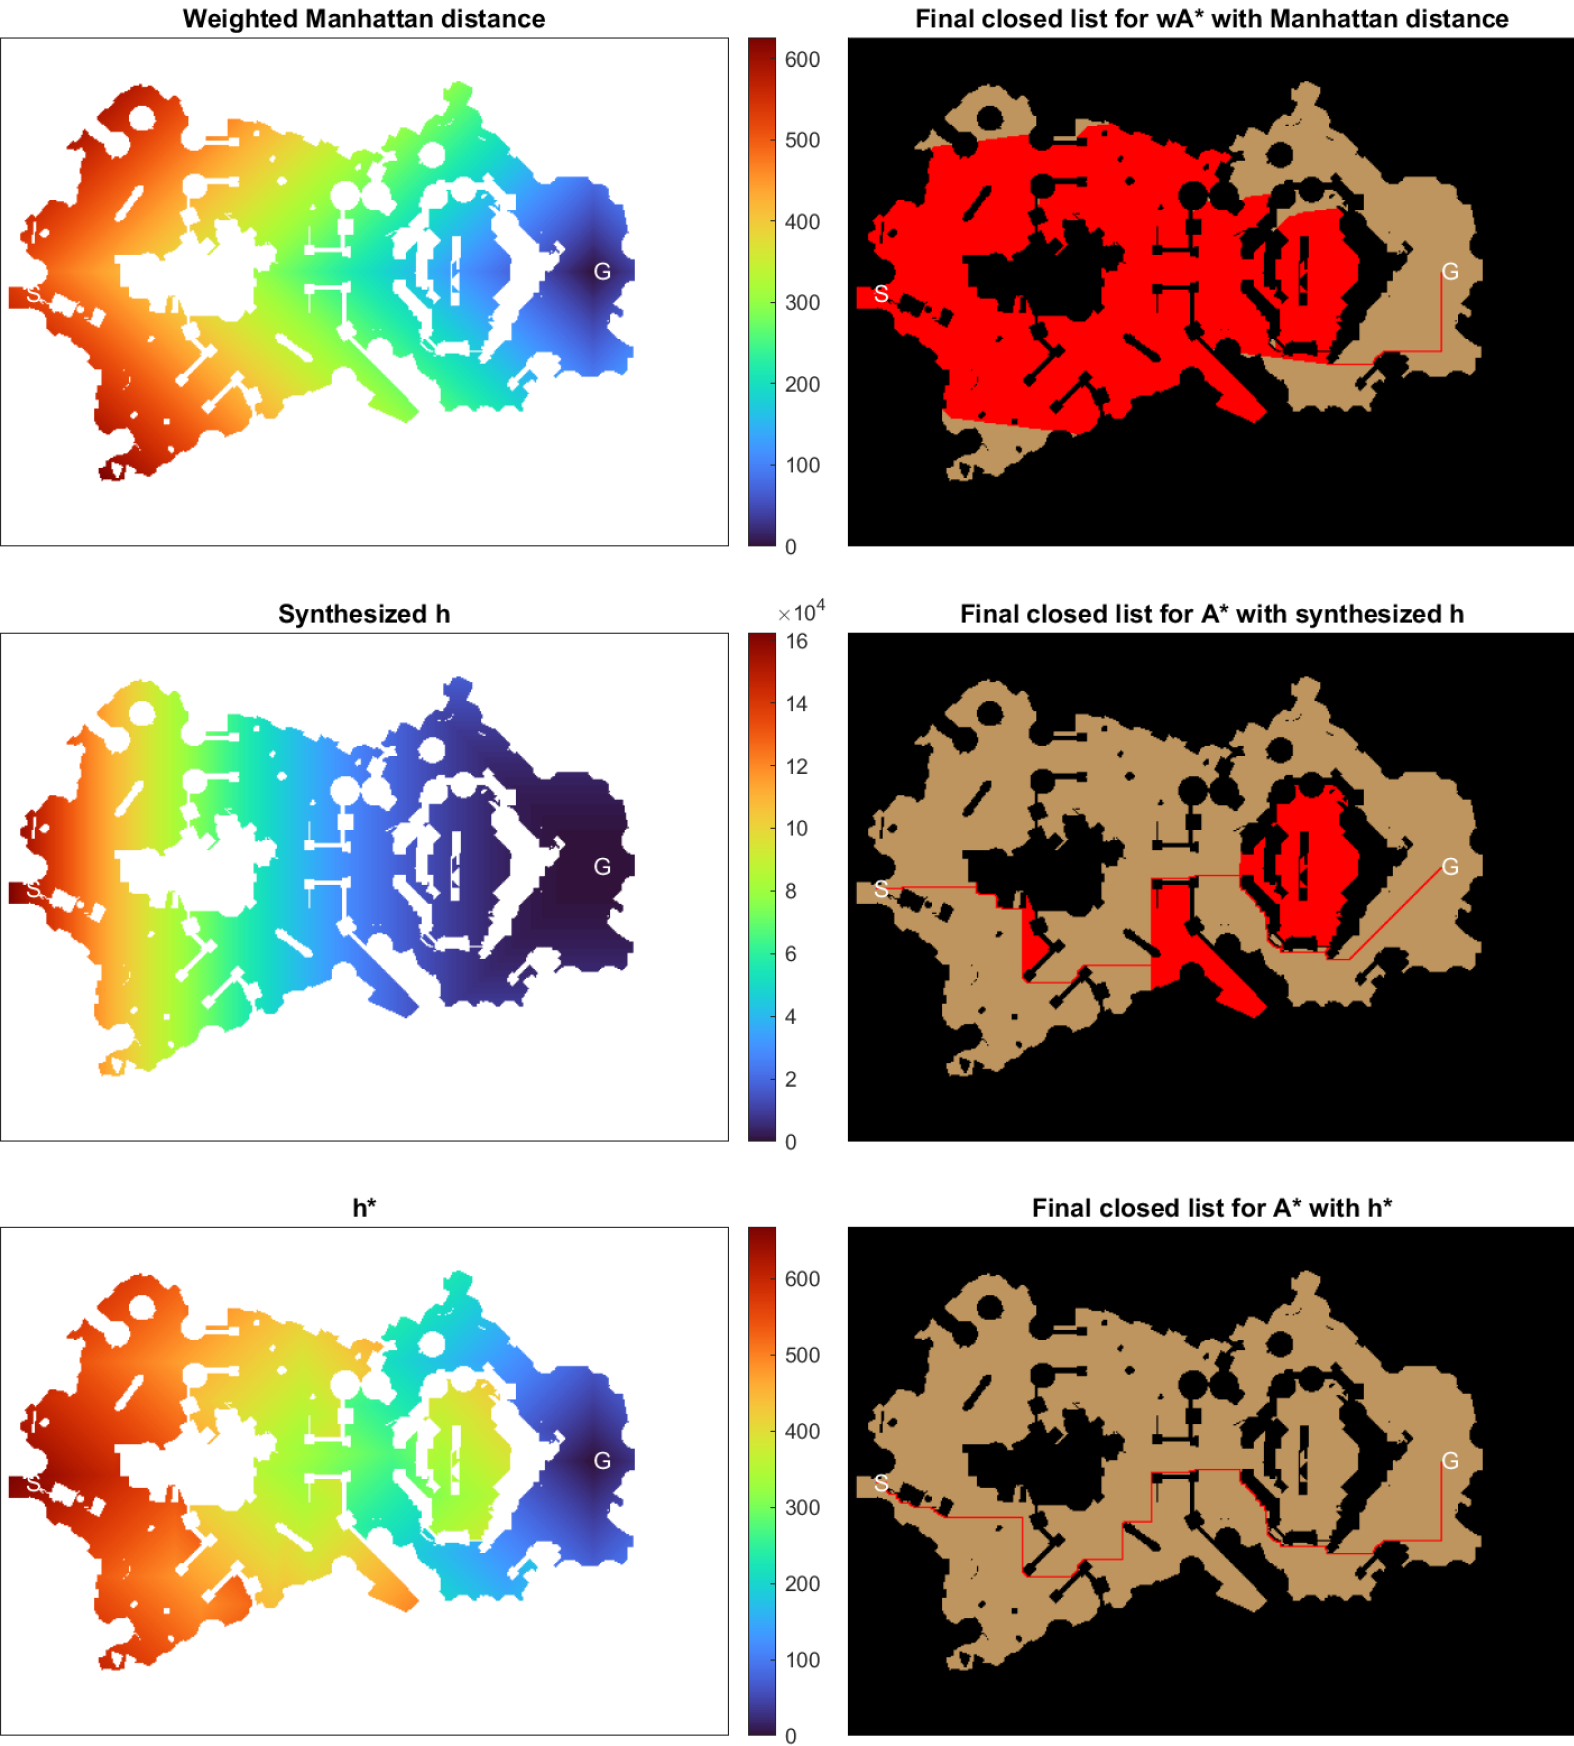
\includegraphics[height=7.5cm]{figs/explainability3.png}
%\caption{Comparing heuristics and final closed lists of the baseline (top row), A* with $h = \max\{\Delta x,\Delta y\}^2$ (middle row) and A* with the perfect heuristic $h^*$ (bottom row). Final closed lists are shown in red. The white {\sf S} and {\sf G} denote the start and goal. The weight $w =  1.2969$ for Manhattan distance was picked to match average suboptimality of $h = \max\{\Delta x,\Delta y\}^2$.}
\label{fig:explainability3}
\end{figure}


\end{frame}


%%%%%%%%%%%%%%%%%%%%%%%%%%%%%%%%%%%%%%%%%%%%%%%%%%%%%%%%%%%%%%%%%%%%%%%%%%%%%%%%

\begin{frame}{Explainability: $\max\{\Delta x,\Delta y\}^2$}

\begin{figure}[htbp]
\centering
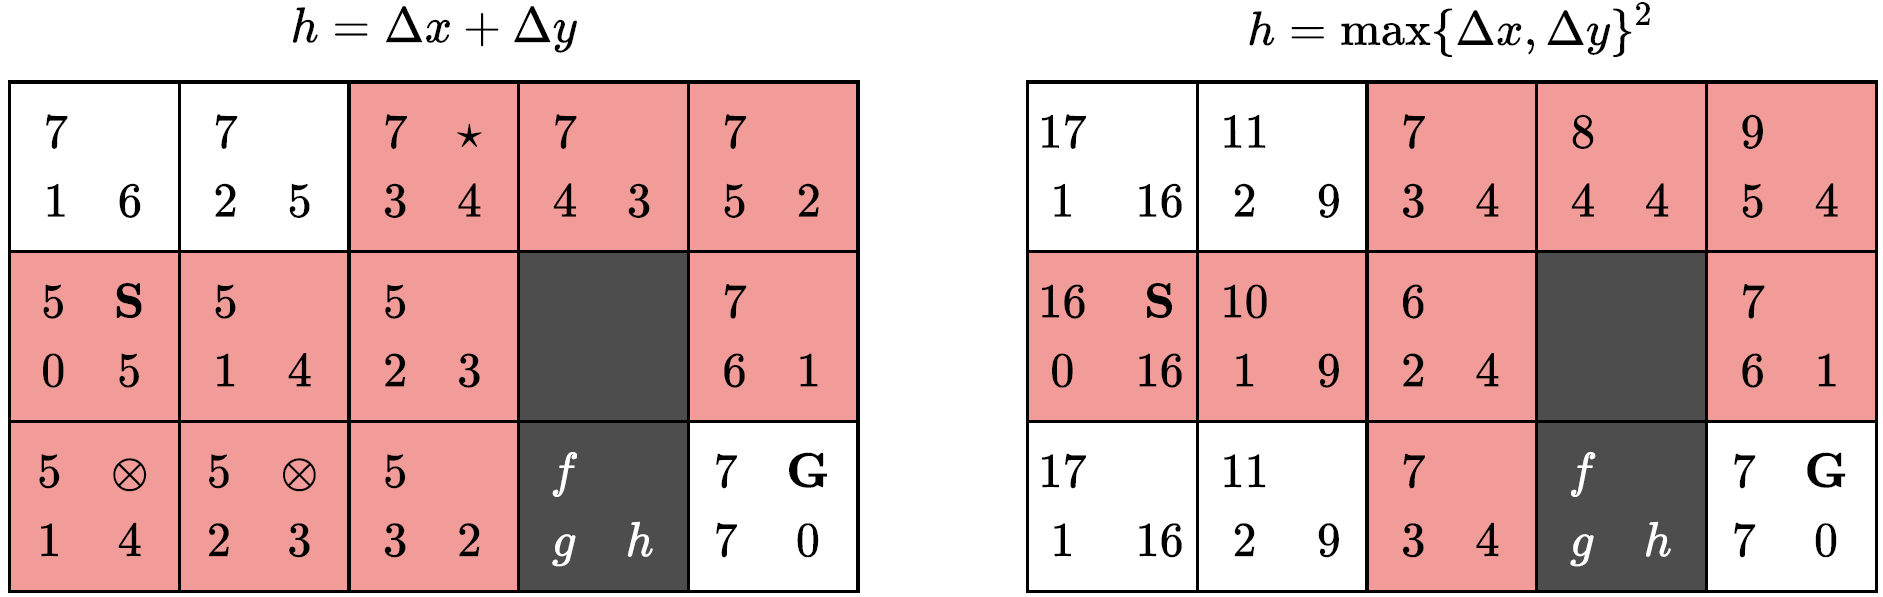
\includegraphics[height=3cm]{figs/synHexample.png}
\vspace{-0.25cm}
\caption{$h=\max\{\Delta x,\Delta y\}^2$ causes A* to hug the wall and expand fewer states than Manhattan distance $\Delta x + \Delta y$}
\label{fig:microExample}
\end{figure}

\vspace{-0.5cm}

\begin{figure}[t]
\centering
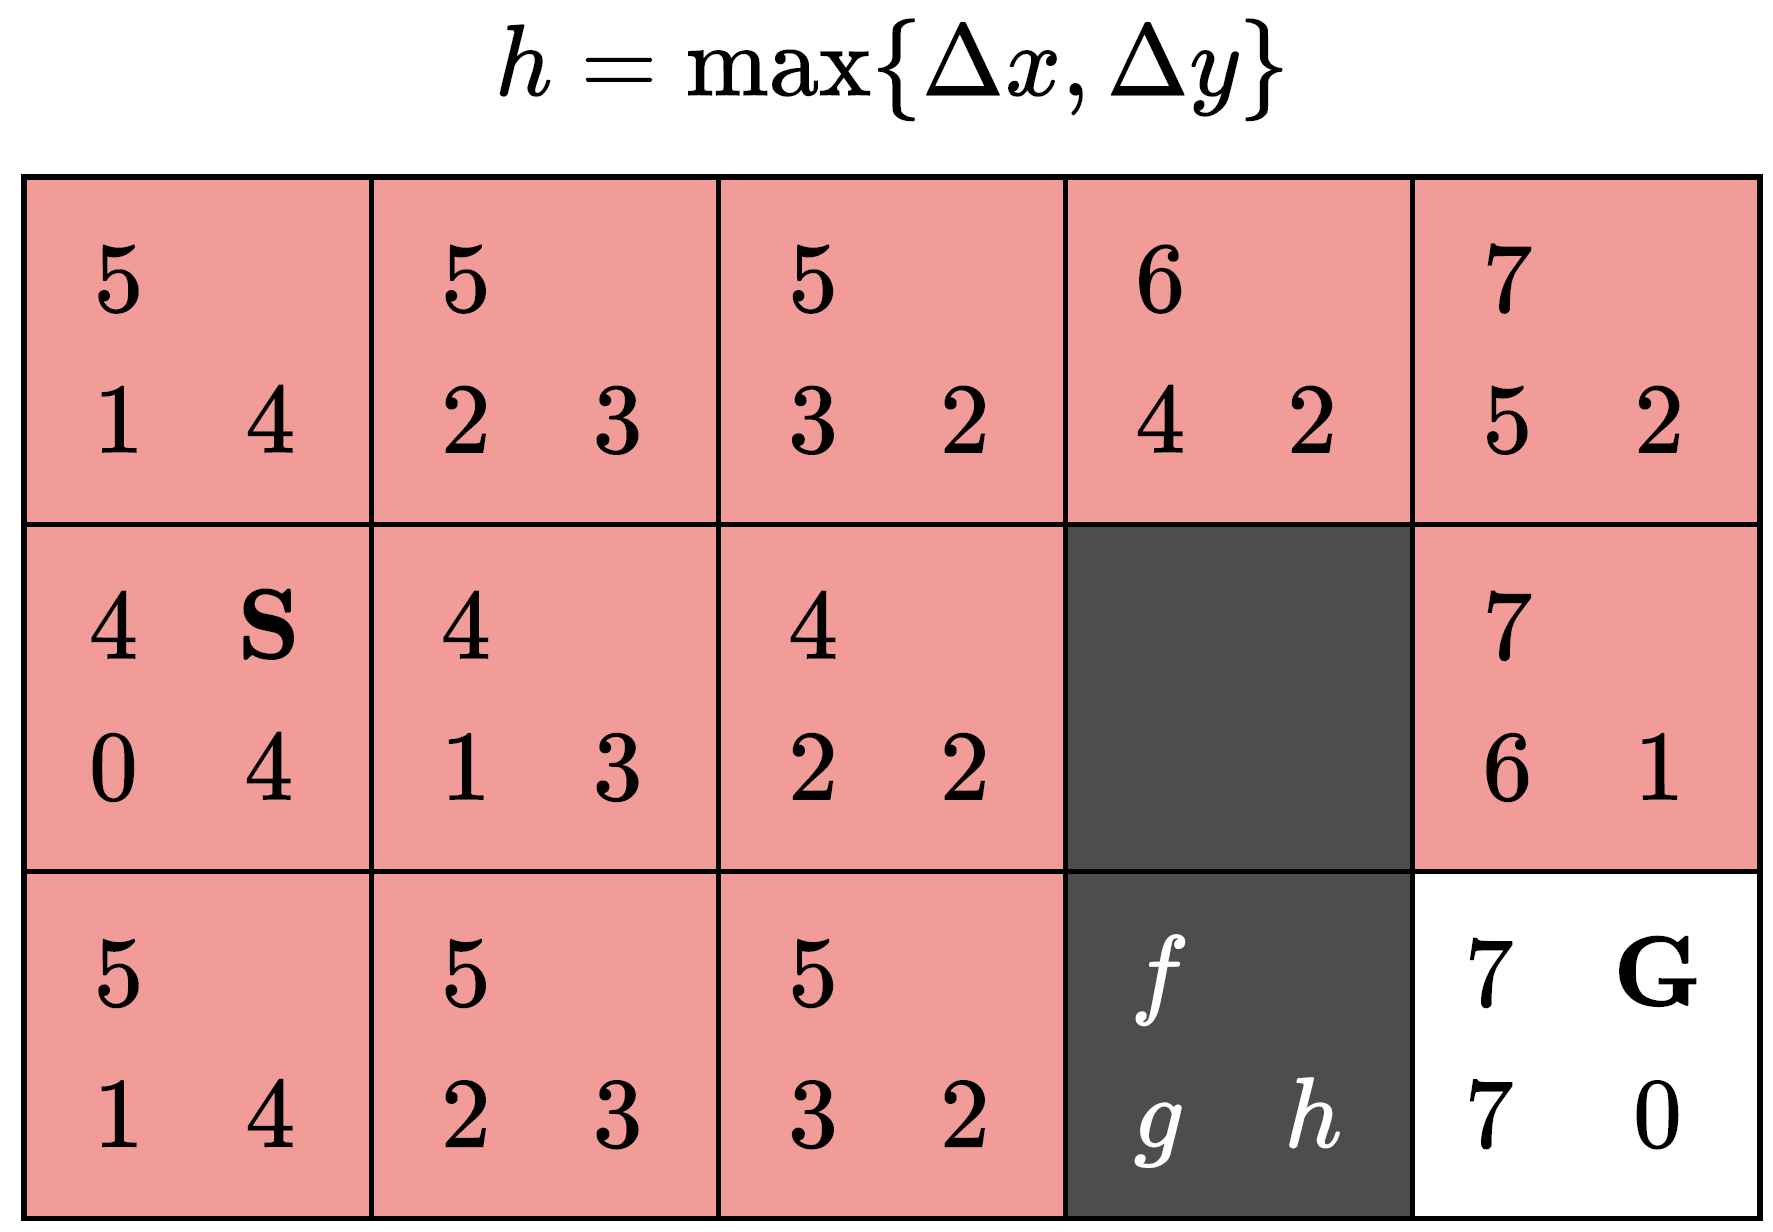
\includegraphics[height=3cm]{figs/synHexample2.png}
\vspace{-0.25cm}
\caption{Removing the square from $h=\max\{\Delta x,\Delta y\}^2$}
\label{fig:microExample2}
\end{figure}


\end{frame}


%%%%%%%%%%%%%%%%%%%%%%%%%%%%%%%%%%%%%%%%%%%%%%%%%%%%%%%%%%%%%%%%%%%%%%%%%%%%%%%%

\begin{frame}{Solution Bounds}

\bei

\ie Human-readable representation of the heuristics $\to$ bound derivation:

\bea 
h(s) &=& \Delta y + \max\left\{6.6 \Delta y,7.7 \Delta x \right\} \nonumber \\ 
&\leq& \Delta y + 6.6 \Delta y + 7.7 \Delta x \nonumber \\ 
&\leq& 7.7 (\Delta y + \Delta x) \nonumber \\ 
&\leq& 7.7 h^*(s) \nonumber
\eea

\medskip

solution suboptimality no worse than $7.7$ times optimal

\eei


\end{frame}


%%%%%%%%%%%%%%%%%%%%%%%%%%%%%%%%%%%%%%%%%%%%%%%%%%%%%%%%%%%%%%%%%%%%%%%%%%%%%%%%

\begin{frame}{Synthesis: Enriched Grammars: {\tt DAO-B}}

\begin{figure}[H]
	\centering
	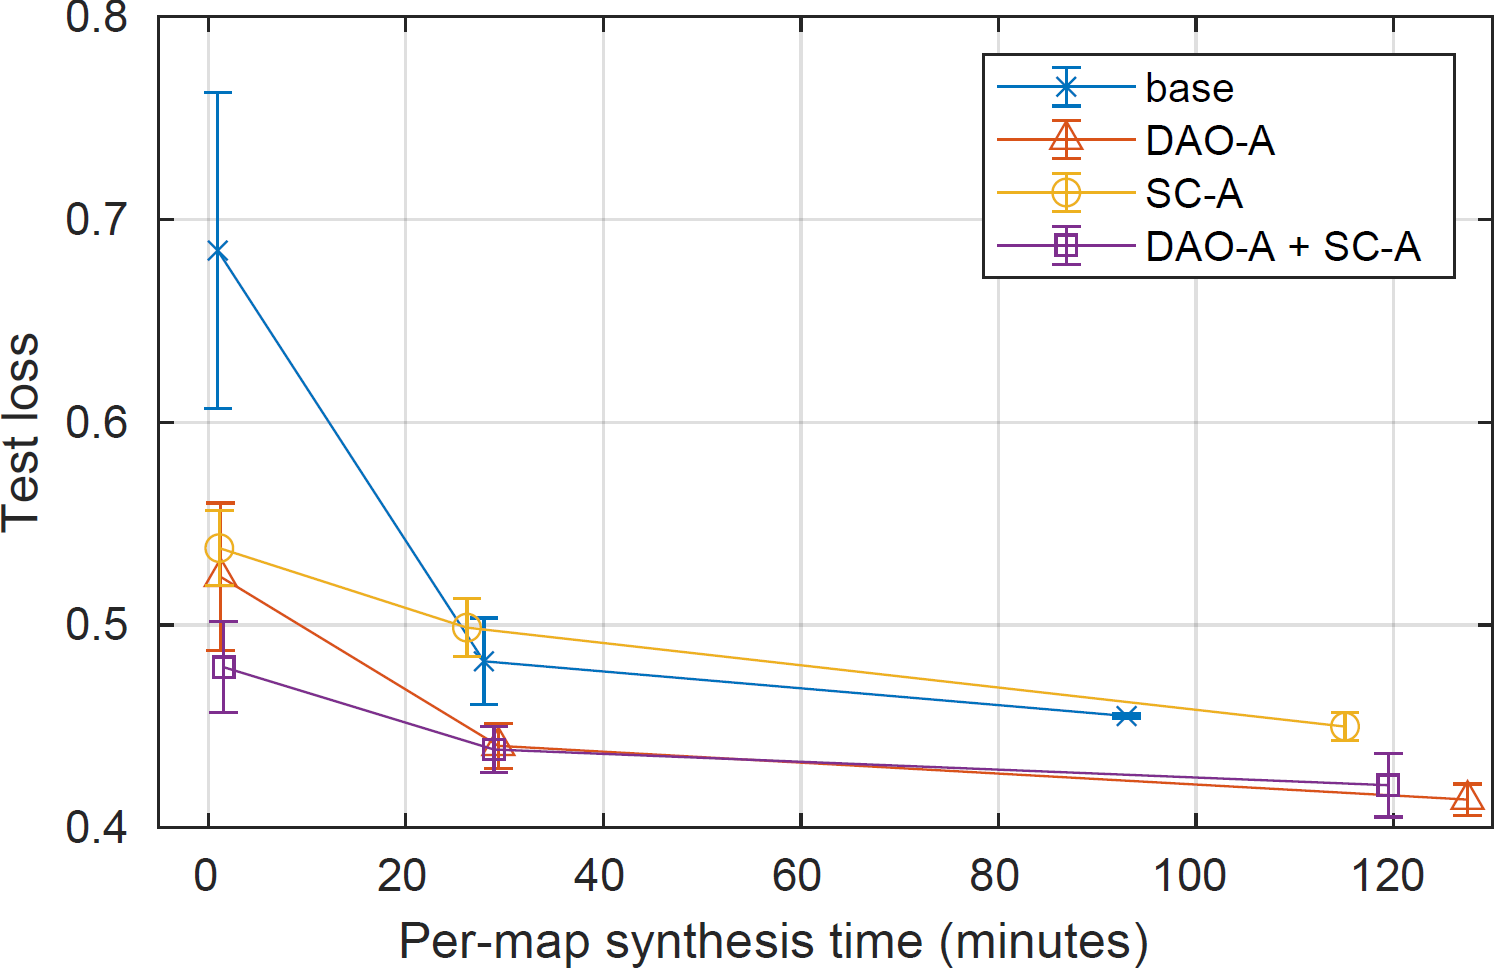
\includegraphics[width=0.75\columnwidth]{figs/bblocks_daoB.png}
\end{figure}


\end{frame}

%%%%%%%%%%%%%%%%%%%%%%%%%%%%%%%%%%%%%%%%%%%%%%%%%%%%%%%%%%%%%%%%%%%%%%%%%%%%%%%%

\begin{frame}{Synthesis: Enriched Grammar: {\tt DAO-B}}

\begin{table}[htbp]
	{%\small
\begin{center}
\begin{tabular}{c|c|l}
			\toprule
			{\bf Map} & {\bf Test loss} & {\bf Heuristic}\\
			\midrule
			{\tt brc100d} & $0.4850$ &
			$\mathbf{f_{3}}$\\
			{\tt brc201d} & $0.4479$ &
			$\min\left\{\min\left\{\mathbf{f_{6}} - x,\mathbf{f_{10}}\right\},\mathbf{f_{7}}\right\}$\\
			{\tt den505d} & $0.4634$ &
			$\max\left\{\max\left\{\frac{\mathbf{f_{1}}}{\mathbf{f_{6}}},\mathbf{f_{5}}\right\} + \Delta x,\mathbf{f_{7}}\right\}$\\
			{\tt lak100c} & $0.3459$ &
			$\mathbf{f_{10}}$\\
			{\tt orz701d} & $0.3943$ &
			$\mathbf{f_{7}}$\\
			{\tt orz702d} & $0.4051$ &
			$\min\left\{\mathbf{f_{3}}^2,\mathbf{f_{1}} + y\right\}$\\
			\bottomrule
	\end{tabular}
\end{center}
}
	\caption{Heuristics synthesized for {\tt DAO-B} with the {\tt DAO-A + SC-A} enriched grammar.}
	\label{tab:h_results_daoB}
\end{table}


\end{frame}


%%%%%%%%%%%%%%%%%%%%%%%%%%%%%%%%%%%%%%%%%%%%%%%%%%%%%%%%%%%%%%%%%%%%%%%%%%%%%%%%

\begin{comment}

\begin{frame}{Synthesis: Enriched Grammars: {\tt SC-B}}

\begin{figure}[H]
	\centering
	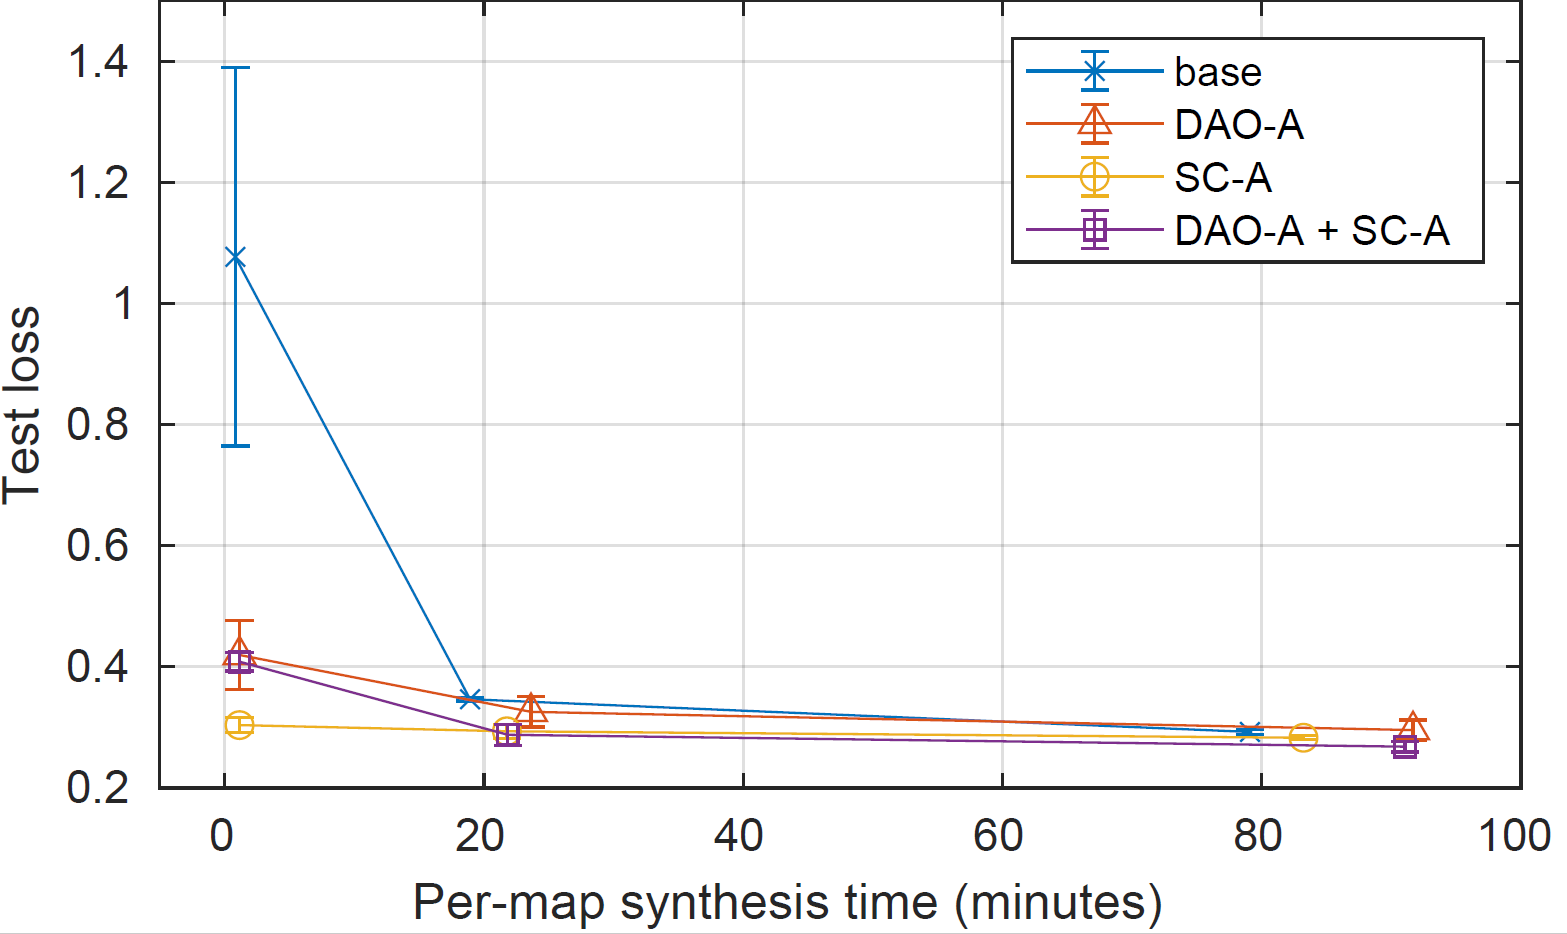
\includegraphics[width=0.8\columnwidth]{figs/bblocks_starcraftB.png}
\end{figure}


\end{frame}

%%%%%%%%%%%%%%%%%%%%%%%%%%%%%%%%%%%%%%%%%%%%%%%%%%%%%%%%%%%%%%%%%%%%%%%%%%%%%%%%

\begin{frame}{Synthesis: Enriched Grammar: {\tt SC-B}}

\begin{table}[htbp]
	{%\small
\begin{center}
\begin{tabular}{c|c|l}
			\toprule
			{\bf Map} & {\bf Test loss} & {\bf Heuristic}\\
			\midrule
			{\tt Aftershock} & $0.2483$ & 
			$\max\left\{\frac{\mathbf{f_{3}}}{1.3},\frac{\mathbf{f_{5}}}{\sqrt{3.1}}\right\}$\\
			{\tt Archipelago} & $0.2209$ &
			$\mathbf{f_{12}}$\\
			{\tt BigGameHunters} & $0.3315$ &
			$\max\left\{\mathbf{f_{3}},\mathbf{f_{5}}\right\}$\\
			{\tt Brushfire} & $0.2190$ &
			$\mathbf{f_{11}} + \Delta y$\\
			{\tt Caldera} & $0.1545$ &
			$\mathbf{f_{11}} + \Delta y$\\
			{\tt CatwalkAlley} & $0.4160$ &
			$\mathbf{f_{9}}$\\
			\bottomrule
	\end{tabular}
\end{center}
}
	\caption{Heuristics synthesized for {\tt SC-B} with the {\tt DAO-A + SC-A} enriched grammar.}
	\label{tab:h_results_scB}
\end{table}


\end{frame}

\end{comment}


%%%%%%%%%%%%%%%%%%%%%%%%%%%%%%%%%%%%%%%%%%%%%%%%%%%%%%%%%%%%%%%%%%%%%%%%%%%%%%%%

\begin{frame}{Portability}

\begin{table}[htbp]
\centering
{\small
\begin{tabular}{c|cc}
\toprule
\diagbox{\bf Synthesis map set}{\bf Test map set} & {\tt DAO-B} & {\tt SC-B} \\
\toprule
{\tt DAO-B} & $\mathbf{0.61}$ & $0.53$ \\
{\tt SC-B} & $0.67$ & $\mathbf{0.36}$ \\
\bottomrule
\end{tabular}
}
\caption{Test loss across map sets. Best values are in bold.}
\label{tab:abstractPortabilityLoss}
\end{table}

\begin{table}[htbp]
\centering
{\small
\begin{tabular}{c|cc}
\toprule
\diagbox{\bf Synthesis map set}{\bf Test map set} & {\tt DAO-B} & {\tt SC-B} \\
\toprule
{\tt DAO-B} & $\mathbf{0.19}$ & $0.27$ \\
{\tt SC-B} & $0.25$ & $\mathbf{0.09}$ \\
\bottomrule
\end{tabular}
}
\caption{Degradation across map sets. Best values bolded.}
\label{tab:abstractPortabilityDegradation}
\end{table}


\end{frame}




%%%%%%%%%%%%%%%%%%%%%%%%%%%%%%%%%%%%%%%%%%%%%%%%%%%%%%%%%%%%%%%%%%%%%%%%%%%%%%%%

\begin{frame}{Current Shortcomings, On-going and Future Work}

\bei

\ie Synthesis: \tcm{basic GAs + probabilistic acceptance}
\bei
\ie \tcg{Bayesian optimization}
\ie \tcg{bottom-up search}
\ie \tcg{advanced GAs}
\eei

\bigskip

\ie Evaluation: \tcm{expensive and rigid}
\bei
\ie \tcg{surrogate fitness functions (e.g., deep ANNs, kNN)}
\ie \tcg{bandits, UCT}
\eei

\bigskip

\ie Domain: \tcm{2D grid pathfinding}
\bei
\ie \tcg{exponential spaces (e.g., combinatorial puzzles)}
\ie \tcg{general planning}
\eei

\eei

\end{frame}

%%%%%%%%%%%%%%%%%%%%%%%%%%%%%%%%%%%%%%%%%%%%%%%%%%%%%%%%%%%%%%%%%%%%%%%%%%%%%%%%

\begin{frame}{Conclusions}

\bei

\ie Automatically synthesized heuristics for A*-driven pathfinding in video games

\medskip

\bei

\ie high performance

\medskip

\ie portability across maps

\medskip

\ie negligible memory footprint

\medskip

\ie human-readable

\medskip

\ie short synthesis time 

\eei

\eei

\end{frame}

%%%%%%%%%%%%%%%%%%%%%%%%%%%%%%%%%%%%%%%%%%%%%%%%%%%%%%%%%%%%%%%%%%%%%%%%%%%%%%%%



\begin{frame}[allowframebreaks]{Bibliography}
\renewcommand*{\bibfont}{\footnotesize}
\printbibliography
\end{frame}

%%%%%%%%%%%%%%%%%%%%%%%%%%%%%%%%%%%%%%%%%%%%%%%%%%%%%%%%%%%%%%%%%%%%%%%%%%%%%%%%

\end{document}



